\documentclass[12pt]{article}
\usepackage{lingmacros}
\usepackage{tree-dvips}
\usepackage{ragged2e}
\usepackage[spanish,es-noshorthands]{babel}
\usepackage[utf8]{inputenc}
\usepackage{amssymb}
\usepackage{tikz}
\usepackage{enumerate}
\usepackage[a4paper, margin = 1.5cm]{geometry}
\usepackage{multicol}
\usetikzlibrary{scopes}
\usepackage{amsmath,amsthm}
\usepackage{amsfonts}
\usepackage{graphicx}

\begin{document}
\title{Resolución C I. Lista 3}
\author{Alvarado Cristo Daniel}
\date{Abril de 2023}
\maketitle

Los presentes ejercicios fueron diseñados para ser resueltos conforme el lector vaya comprendiendo los conceptos y resultados dados en la teoría, si se tiene alguna duda sobre alguno(s) de ellos se recomienda sea disipada de inmediato. Se sugiere al lector redactar, según su criterio, una guía que contenga aquellos conceptos y resultados del capítulo que considere más importantes y/o útiles como referencia
rápida de consulta para la solución de los problemas.

%\renewcommand\qedsymbol{$\square$}%

\def\proof{\paragraph{Demostración:\\}}
\def\endproof{\hfill$\blacksquare$}

\def\sol{\paragraph{Solución:\\}}
\def\endsol{\hfill$\square$}

\renewcommand{\labelenumi}{\textbf{3.\theenumi.}}
\renewcommand{\labelenumii}{\textbf{\Roman{enumii}.}}
\providecommand{\abs}[1]{\left| #1 \right|}
\newcommand{\cf}[3]{\ensuremath{#1:#2\rightarrow#3}}

\begin{enumerate}
    \item Sea
    \begin{equation*}
        f(x)=\left\{
            \begin{array}{lcr}
                1 & \textup{ si } & -3\leq x<-1\\
                \abs{x} & \textup{ si } & -1\leq x<0\\
                1 & \textup{ si } & x=1/2\\
                x^2 & \textup{ si } & 1\leq x<3 
            \end{array}
        \right.
    \end{equation*}
    \begin{enumerate}
        \item ¿\textbf{Cuál} es el dominio de $f$? \textbf{Calcule}: $f(2),f(3/2),f(\sqrt{2}),f(-1/2),f(-\sqrt{2}/2),f(-2)$. \textbf{Bosqueje} la gráfica de $f$.
        \item Defina $h(x)=f(x+1)$. \textbf{Determine} el dominio de $h$. \textbf{Calcule}: $h(1),h(1/2),h(\sqrt{2}-1),h(-3/2),h(-1-\sqrt{2}/2)$ y $h(-3)$. \textbf{Bosqueje} la gráfica de $h$. ¿Existe alguna relación entre la gráfica de $f$ y la gráfica de $h$? \textbf{Explique}.
        \item Defina $k(x)=f(x)+1$. \textbf{Determine} el dominio de $k$. \textbf{Calcule} $k(2),k(3/2),k(\sqrt{2}),k(-1/2)$ ,$k(-\sqrt{2}/2)$ y $k(-2)$. \textbf{Bosqueje} la gráfica de $k$. ¿Existe alguna relación entre la gráfica de $f$ y la gráfica de $k$? \textbf{Explique}.
    \end{enumerate}

    \begin{sol}
        De (i): Los posibles valores que $f$ toma son cuando $-3\leq x <-1$, $-1\leq x<0$, $x=\frac{1}{2}$ o $1\leq x<3$, esto es, el dominio de $f$ es el conjunto:
        \begin{equation*}
            D_f=[-3,0[\cup\left\{\frac{1}{2}\right\}\cup[1,3[
        \end{equation*}
        y, se tiene que:
        \begin{itemize}
            \item $f(2)=2^2=4$.
            \item $f(3/2)=\left(3/2\right)^2=9/4$.
            \item $f(\sqrt{2})=\left(\sqrt{2} \right)^2=2$.
            \item $f(-1/2)=\abs{-1/2}=1/2$.
            \item $f(-\sqrt{2}/2)=1$.
            \item $f(-2)=1$.
        \end{itemize}
        La gráfica de $f$ está dada como se muestra en la figura 1:
        \begin{figure}
            \begin{center}
                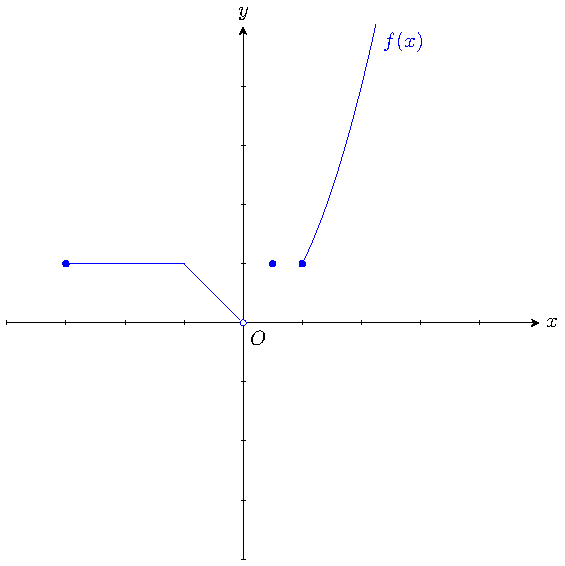
\includegraphics[scale=1]{images/3_1.pdf}
            \end{center}
            \caption{Plot de la función $f$.}
        \end{figure}

        De (ii): El dominio de $h$ son los puntos $x\in\mathbb{R}$ para los cuales $f(x+1)$ está definido, es decir que $x+1\in D_f$, por tanto el dominio de $h$ es el conjunto
        \begin{equation*}
            D_h=[-4,-1[\cup\left\{-\frac{1}{2}\right\}\cup[0,2[
        \end{equation*}
        y, se tiene que
        \begin{itemize}
            \item $h(1)=f(1+1)=2^2=4$.
            \item $h(1/2)=f(1/2+1)=f(3/2)=\left(3/2\right)^2=9/4$.
            \item $h(\sqrt{2}-1)=f(\sqrt{2})=\left(\sqrt{2} \right)^2=2$.
            \item $h(-3/2)=f(-1/2)=\abs{-1/2}=1/2$.
            \item $h(-1-\sqrt{2}/2)=f(-\sqrt{2}/2)=1$.
            \item $h(-3)=f(-2)=1$.
        \end{itemize}
        La gráfica de $h$ está dada como se muestra en la figura 2.

        \begin{figure}
            \begin{center}
                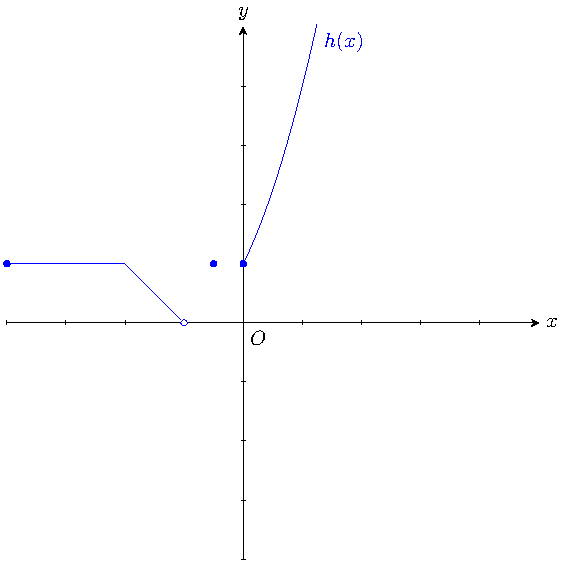
\includegraphics[scale=1]{images/3_1_2.pdf}
            \end{center}
            \caption{Plot de la función $h$.}
        \end{figure}
        
        donde, podemos observar que lo que se hace con respecto a la gráfica de $f$, es recorrer la gráfica en el sentido horizontal una unidad hacia la izquierda.

        De (iii): El dominio de $k$ son los posibles valores para los que $f(x)+1$ está definido, es decir para cuando $f$ está definido, por lo cual
        \begin{equation*}
            D_k=D_f=[-3,0[\cup\left\{\frac{1}{2}\right\}\cup[1,3[
        \end{equation*}
        y, se tiene que
        \begin{itemize}
            \item $k(2)=f(2)+1=2^2+1=5$.
            \item $k(3/2)=f(3/2)+1=\left(3/2\right)^2+1=13/4$.
            \item $k(\sqrt{2})=f(\sqrt{2})+1=\left(\sqrt{2} \right)^2+1=3$.
            \item $k(-1/2)=f(-1/2)+1=\abs{-1/2}+1=3/2$.
            \item $k(-\sqrt{2}/2)+1=f(-\sqrt{2}/2)+1=2$.
            \item $k(-2)=f(-2)+1=2$.
        \end{itemize}
        La gráfica de $k$ está dada como se muestra en la figura 3:
        \begin{figure}
            \begin{center}
                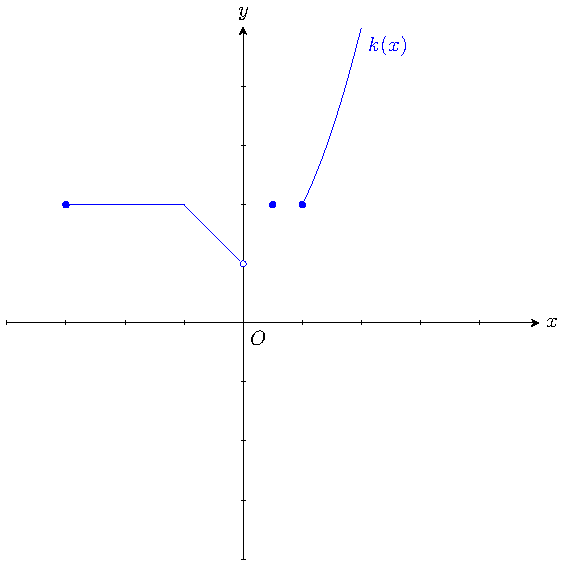
\includegraphics[scale=1]{images/3_1_3.pdf}
            \end{center}
            \caption{Plot de la función $k$.}
        \end{figure}

        donde, podemos observar que lo que se hace con respecto a la gráfica de $f$, es recorer la gráfica verticalmente una unidad hacia arriba.
    \end{sol}

    \item \textbf{Analice} la variación de las siguientes funciones (dominio natural, raíces, intervalos de monotonía, comportamiento en los extremos de dichos intervalos, cuadro de variación y gráfica):
    \begin{enumerate}
        \item $f(x)=x^2+3x$.
        \item $g(x)=\frac{x-1}{2x+2}$.
        \item $h(x)=\abs{x}$.
    \end{enumerate}

    \begin{sol}
        De (i): La gráfica de la función $f$ es la de la mostrada en la figura 4:
        \begin{figure}
            \begin{center}
                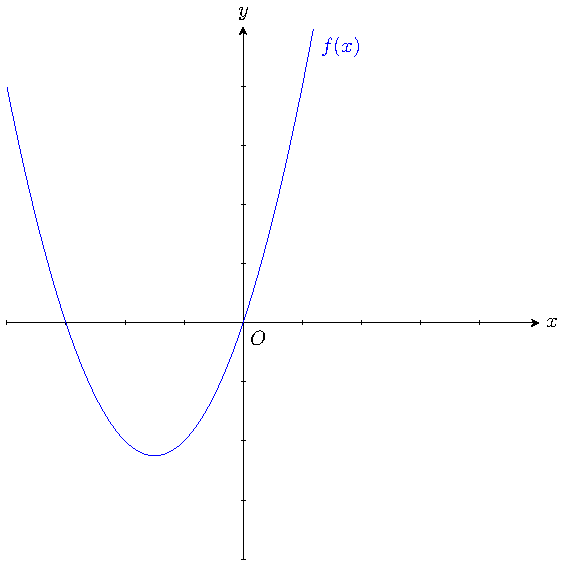
\includegraphics[scale=1]{images/3_2_1.pdf}
            \end{center}
            \caption{Plot de la función $f$.}
        \end{figure}

        De (ii): La gráfica de la función $g$ es la de la mostrada en la figura 5:
        \begin{figure}
            \begin{center}
                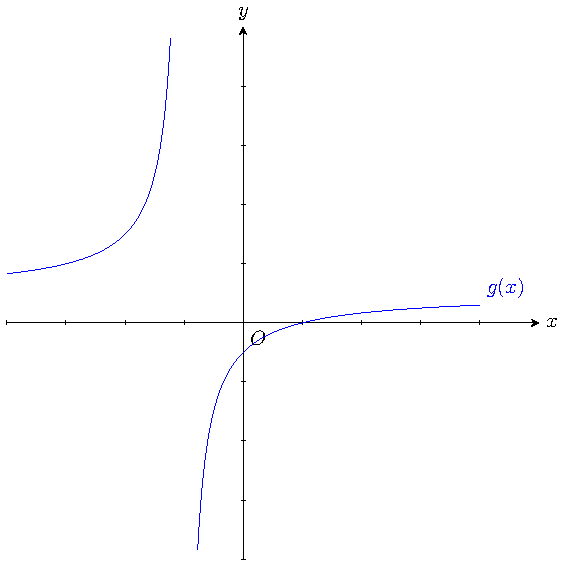
\includegraphics[scale=1]{images/3_2_2.pdf}
            \end{center}
            \caption{Plot de la función $g$.}
        \end{figure}

        De (iii): La gráfica de la función $h$ es la de la mostrada en la figura 6:
        \begin{figure}
            \begin{center}
                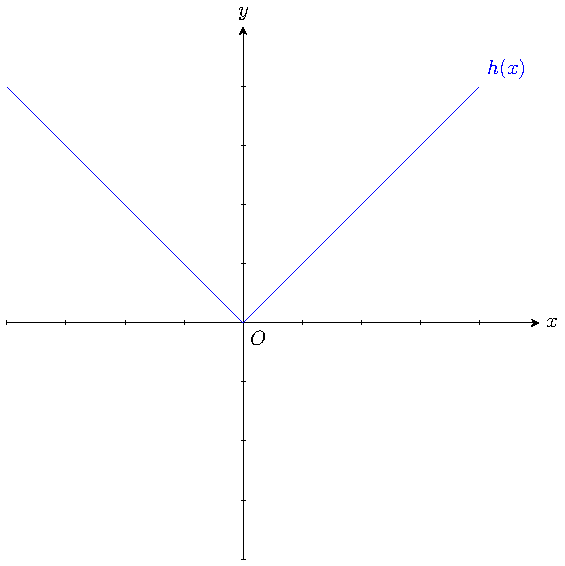
\includegraphics[scale=1]{images/3_2_3.pdf}
            \end{center}
            \caption{Plot de la función $h$.}
        \end{figure}

    \end{sol}

    \item \textbf{Determine} el dominio natrual de las siguientes funciones:
    \begin{enumerate}
        \item $x\mapsto \sqrt{3-x^2}$.
        \item $y\mapsto\sqrt{1-\sqrt{1-y^2}}$.
        \item $\omega\mapsto\frac{1}{\omega-1}+\frac{1}{\omega-2}$.
        \item $u\mapsto\sqrt{1-u^2}+\sqrt{u^2-1}$.
        \item $t\mapsto\sqrt{1-t}+\sqrt{t-2}$.
    \end{enumerate}

    \begin{sol}
        De (i): La función $x\mapsto\sqrt{3-x^2}$ está definida si y sólo si $3-x^2\geq0$, esto es $x^2\leq3$ lo cual ocurre si y sólo si $-\sqrt{3}\leq x\leq\sqrt{3}$.

        Así, el dominio natural de esta función es $[-\sqrt{3},\sqrt{3}]$.

        De (ii): La función $y\mapsto\sqrt{1-\sqrt{1-y^2}}$ está definida si y sólo si $1-\sqrt{1-y^2}\geq0$, es decir si y sólo si $\sqrt{1-y^2}\leq1$, esto es cuando $0\leq1-y^2\leq 1$ y,
        \begin{equation*}
            \begin{split}
                0\leq1-y^2\leq 1&\iff 0\leq y^2\leq1\\
                &\iff -1\leq y\leq1\\
            \end{split}
        \end{equation*}
        por tanto, el dominio natural de esta función es $[-1,1]$.

        De (iii): La función $\omega\mapsto\frac{1}{\omega-1}+\frac{1}{\omega-2}$ está definida cuando $\omega-1\neq 0$ y $\omega-2\neq0$, esto es:
        \begin{equation*}
            \omega\neq1,2
        \end{equation*}
        luego, el dominio natural de esta función es $\mathbb{R}\backslash\left\{1,2 \right\}$.

        De (iv): La función $u\mapsto\sqrt{1-u^2}+\sqrt{u^2-1}$ está definida si y sólo si $1-u^2,u^2-1\geq0$, esto es:
        \begin{equation*}
            1\leq u^2\quad\textup{y}\quad u^2\geq1
        \end{equation*}
        y, esto sólo ocurre cuando $u=\pm1$. Por tanto, el dominio natrual de $f$ es $\left\{-1,1 \right\}$.

        De (v): 
    \end{sol}

    \item \begin{enumerate}
        \item \textbf{Muestre} que si $\abs{x-1}\leq 1$, entonces $\abs{x^2+3x-4}\leq 6\abs{x-1}$.
        \item Sea $\varepsilon>0$. Use el inciso anterior para \textbf{probar} que si $\abs{x-1}<\min\left\{1,\frac{\varepsilon}{6} \right\}$, entonces $\abs{x^2+3x-4}\leq\varepsilon$. Aplique la definición de límite para \textbf{concluir} que
        \begin{equation*}
            \lim_{x\rightarrow1}x^2+3x=4
        \end{equation*}
    \end{enumerate}

    \begin{proof}
        De (i): Sea $x\in\mathbb{R}$ tal que $\abs{x-1}\leq 1$, entonces $\abs{x}-1\leq1\Rightarrow \abs{x}\leq2$. Con esto, se sigue que:
        \begin{equation*}
            \begin{split}
                \abs{x^2+3x-4}&=\abs{(x+4)(x-1)}\\
                &=\abs{x-1}\abs{x+4}\\
                &\leq\abs{x-1}\left(\abs{x}+4\right) \\
                &\leq\abs{x-1}\left(2+4\right)\\
                &\leq6 \abs{x-1}\\
                \Rightarrow \abs{x^2+3x-4}&\leq6 \abs{x-1}\\ 
            \end{split}
        \end{equation*}

        De (ii): Sea $x\in\mathbb{R}$ tal que $\abs{x-1}<\min\left\{1,\frac{\varepsilon}{6} \right\}$, es decir que
        \begin{equation*}
            \abs{x-1}<1\quad\textup{y}\quad\abs{x-1}<\frac{\varepsilon}{6}
        \end{equation*}
        por la parte (i), se sigue que $\abs{x^2-3x-4}\leq 6\abs{x-1}$ y, por la segunda desigualdad, se sigue que
        \begin{equation*}
            \abs{x^2-3x-4}\leq 6\abs{x-1}<6\cdot\frac{\varepsilon}{6}=\varepsilon
        \end{equation*}
        por tanto, $\abs{x^2-3x-4}<\varepsilon$. Ahora, como para todo $\varepsilon>0$ existe $\delta=\min\left\{1,\frac{\varepsilon}{6} \right\}>0$ tal que
        \begin{equation*}
            \forall x\in\mathbb{R},x\neq1\textup{ tal que } \abs{x-1}<\delta \Rightarrow \abs{x^2-3x-4}<\varepsilon
        \end{equation*}
        se sigue que
        \begin{equation*}
            \lim_{x\rightarrow 1}x^2-3x=4
        \end{equation*}
    \end{proof}

    \item Usando la definición de límite, \textbf{demuestre} las afirmaciones siguientes.
    \begin{enumerate}
        \item $\lim_{x\rightarrow-1}\abs{x^3}=1$.
        \item $\lim_{x\rightarrow1}f(x)=1$, donde $f(x)=\left\{\begin{array}{lcr}
            \sqrt{x} & \textup{ si } & 0\leq x<1\\
            x^2 & \textup{ si } & 1 <x\leq 2 \\
        \end{array} \right.$
        \item ¿Existe $\lim_{x\rightarrow0}f(x)$, donde $f(x)=\left\{\begin{array}{lcr}
            x^3-2x^2+x & \textup{ si } & x\neq0 \\
            1 & \textup{ si } & x=0 \\
        \end{array} \right.$? \textbf{Justifique}.
    \end{enumerate}

    \begin{proof}
        De (i): Sea $\varepsilon>0$. Observemos que si $\abs{x+1}\leq1$:
        \begin{equation*}
            \begin{split}
                \abs{\abs{x^3}-1}&\leq\abs{-x^3-1}\\
                &\leq\abs{(x+1)(x^2-x+1)}\\
                &\leq\abs{x+1}\abs{x^2-x+1}\\
            \end{split}
        \end{equation*}
        entonces, como $\abs{x}-\abs{-1}\leq\abs{x-(-1)}$, se sigue que $\abs{x}\leq2$. Luego
        \begin{equation*}
            \begin{split}
                \abs{x^2+x+1}&\leq\abs{x^2}+\abs{x}+1\\
                &\leq 2^2+2+1\\
                &=7\\
                \Rightarrow \abs{\abs{x^3}-1}&\leq7\abs{x+1}
            \end{split}
        \end{equation*}
        tomemos entonces $\delta=\min\left\{1,\frac{\varepsilon}{7}\right\}>0$. Se tiene entonces que si $\abs{x+1}<\delta$, por lo anterior, que 
        \begin{equation*}
            \abs{\abs{x^3}-1}\leq7\abs{x+1}
        \end{equation*}
        además, $\abs{x+1}<\frac{\varepsilon}{7}$, por lo cual
        \begin{equation*}
            \begin{split}
                \abs{\abs{x^3}-1}&<7\cdot\frac{\varepsilon}{7}\\
                &=\varepsilon\\
                \Rightarrow \abs{\abs{x^3}-1}<\varepsilon \\
                \therefore \abs{x-(-1)}<\delta\Rightarrow \abs{\abs{x^3}-1}<\varepsilon \\
            \end{split}
        \end{equation*}
        Luego, de la definición de límite por $\varepsilon-\delta$ se sigue que
        \begin{equation*}
            \lim_{ x\rightarrow-1}\abs{x^3}=1
        \end{equation*}

        De (ii): 
    \end{proof}

    \item Usando primero la definición de límite, luego algunos teoremas sobre límites y finalmente la caracterización de límites con sucesiones, \textbf{determine} los límites siguientes.
    \begin{enumerate}
        \item $\lim_{t\rightarrow-4}\frac{t^2-t-20}{t+4}$.
        \item $\lim_{y\rightarrow3}\frac{y^2-9}{y^2-2y-3}$.
        \item $\lim_{x\rightarrow1}\left(\frac{1}{1-x}-\frac{x^3-x^2-2}{x^2-1}\right)$.
        \item $\lim_{x\rightarrow0}\frac{1}{3x}\left(\frac{1}{8+x}-\frac{1}{8}\right)$.
        \item $\lim_{x\rightarrow0}\frac{1}{x^2}\left(\frac{2}{x-5}-\frac{2}{x^2+x-5} \right)$.
    \end{enumerate}

    \item Suponga que no existen los límites $\lim{x\rightarrow a}f(x)$ y $\lim{x\rightarrow a}g(x)$. ¿Pueden existir $\lim{x\rightarrow a}(f(x)+g(x))$ ó $\lim{x\rightarrow a}f(x)g(x)$? \textbf{Justifique} formalmente sus respuestas o dando contraejemplos.
    \item \begin{enumerate}
        \item \textbf{Demuestre} que si exiten los límites $\lim{x\rightarrow a}(f(x)+g(x))$ y $\lim{x\rightarrow a}f(x)$, entonces también existe $\lim{x\rightarrow a}g(x)$.
        \item \textbf{Pruebe} que si existen los límites $\lim{x\rightarrow a}f(x)g(x)$ y, además, $\lim{x\rightarrow a}f(x)\neq 0$, entonces también existe $\lim{x\rightarrow a}g(x)$.
    \end{enumerate}
    \item Suponga que exista el límite $\lim{x\rightarrow a}f(x)g(x)$ y, además, $\lim{x\rightarrow a}f(x)=0$. ¿Puede existir $\lim{x\rightarrow a}g(x)$? \textbf{Justifique} formalmente sus respuestas o dando contraejemplos.
    \item \begin{enumerate}
        \item \textbf{Pruebe} que si $\abs{x-2}\leq1$, entonces $\abs{x^2+3x-1}\geq1$.
        \item Sea $\delta>0$. Use el inciso anterior para \textbf{probar} que si $x=\min\left\{5/2,2+\delta/2 \right\}$, entonces $\abs{x^2+3x-1}\geq1$. Aplique la definición de límite para \textbf{concluir} que $\lim_{x\rightarrow2}x^2+3x\neq1$.
    \end{enumerate}
    \item Considere las funciones $j(x)=x$, $s(x)=x^2$ y $h(x)=\sqrt{\abs{x}}$, para todo $x\in\mathbb{R}$.
    \begin{enumerate}
        \item \textbf{Determine} el conjunto de todos los $x\in\mathbb{R}$ para los que se cumpla que $s(x)\leq j(x)$ y \textbf{haga} un dubujo en donde aparezcan simultáneamente las gráficas de $s$ y $j$.
        \item \textbf{Determine} el conjunto de todos los $x\in\mathbb{R}$ para los que se cumpla que $h(x)\leq s(x)$ y \textbf{haga} un dubujo en donde aparezcan simultáneamente las gráficas de $h$ y $s$.
        \item \textbf{Determine} el conjunto de todos los $x\in\mathbb{R}$ para los que se cumpla que $j(x)\leq h(x)$ y \textbf{haga} un dubujo en donde aparezcan simultáneamente las gráficas de $j$ y $h$.
    \end{enumerate}
    \item Sea $S\subseteq\mathbb{R}$. Dadas dos funciones $\cf{f,g}{S}\mathbb{R}$ se define la \textbf{envoltura superior} de $f$ y $g$, como la función $\cf{\max\left(f,g\right)}{S}{\mathbb{R}}$ dada por
    \begin{equation*}
        \max\left(f,g\right)(x)=\max\left(f(x),g(x)\right),\quad\forall x\in S
    \end{equation*}
    y, la \textbf{envoltura inferior} de $f$y $g$ como la función $\cf{\min\left(f,g\right)}{S}{\mathbb{R}}$ dada por
    \begin{equation*}
        \min\left(f,g\right)(x)=\min\left(f(x),g(x)\right),\quad\forall x\in S
    \end{equation*}
    \begin{enumerate}
        \item Reconsidere las funciones $\cf{j,s,h}{\mathbb{R}}{\mathbb{R}}$ del problema anterior. \textbf{Bosqueje} la gráfica de las funciones $\max(j,s),\min(j,s),\max(s,h),\min(s,h),\max(j,h),\min(j,h)$.
        \item \textbf{Escriba} las funciones $\max(f,g)$ y $\min(f,g)$ en términos de $f$ y $g$ y del valor absoluto.
    \end{enumerate}
    \item Aplique el teorema de comparación y/o el tereoma de álgebra de límites para \textbf{calcular} los límites siguientes.
    \begin{enumerate}
        \item $\lim_{x\rightarrow0}\frac{\tan^2x}{x}$.
        \item $\lim_{x\rightarrow a}\left[\frac{\sen x-\sen a}{x-a} \right]$, donde $a\in\mathbb{R}$.
        \item $\lim_{x\rightarrow0}\sqrt{\abs{x}}\sen\left(\frac{1}{x}\right)$.
        \item Sean $\cf{f,g}{S}{\mathbb{R}}$ dos funciones y $a\in\mathbb{R}$. Suponga que $g$ es acotada en $S$ y que $\lim_{x\rightarrow a}f(x)=0$. \textbf{Demuestre} que
        \begin{equation*}
            \lim_{x\rightarrow a}f(x)g(x)=0
        \end{equation*}
    \end{enumerate}
    \item Use el teorema sobre la caracterización de límites de funciones por medio de sucesiones en los problemas siguientes.
    \begin{enumerate}
        \item \textbf{Calcule} $\lim_{x\rightarrow-2}\sqrt[3]{\frac{x-1}{2x+2}}$.
        \item \textbf{Calcule} $\lim_{x\rightarrow-3}\sqrt[3]{\abs{x}^3}$.
        \item \textbf{Muestre} que no existe $\lim_{x\rightarrow0}\sen\left(\frac{1}{x}\right)$.
        \item \textbf{Muestre} que no existe $\lim_{x\rightarrow2}E(x)$, donde $E$ es la función parte entera.
        \item \textbf{Muestre} que no existe $\lim_{x\rightarrow2}f(x)$, donde $f(x)=\left\{\begin{array}{lcr}
            \sqrt{x} & \textup{ si } & 0\leq x<2\\
            x^3 & \textup{ si } & 2<x\leq3 \\
        \end{array} \right.$.
        \item \textbf{Muestre} que no existe $\lim_{x\rightarrow a}f(x)$, donde $f$ es la función de Dirichlet y $a\in\mathbb{R}$ es arbitrario.
    \end{enumerate}
    \item Usando primero la definición de límite y después el teorema sobre caracterizació nde límites de funciones por medio de sucesiones, \textbf{pruebe} que:
    \begin{enumerate}
        \item $\lim_{x\rightarrow1}\frac{x-1}{2x+2}\neq 3$.
        \item $\lim_{x\rightarrow 2}\abs{x}\neq -1$.
    \end{enumerate}
    \item Considere la función
    \begin{equation*}
        f(x)=\left\{
            \begin{array}{lcr}
                -x & \textup{ si } & -3\leq x\leq-1\\
                x^3 & \textup{ si } & -1< x<1\\
                \sqrt{x} & \textup{ si } & 1<x\leq3 \\
                \frac{1}{3-x}+\sqrt{3} & \textup{ si } & 3<x\\ 
            \end{array}
        \right.
    \end{equation*}
    \begin{enumerate}
        \item \textbf{Bosqueje} la gráfica de $f$.
        \item \textbf{Calcule} $\lim_{x \rightarrow-1^-}f(x)$ y $\lim_{x \rightarrow-1^+}f(x)$ ¿Existe $\lim_{x \rightarrow-1}f(x)$?
        \item \item \textbf{Calcule} $\lim_{x \rightarrow1^-}f(x)$ y $\lim_{x \rightarrow1^+}f(x)$ ¿Existe $\lim_{x \rightarrow1}f(x)$?
        \item ¿Existen $\lim_{x \rightarrow3^-}f(x)$, $\lim_{x \rightarrow3^+}f(x)$ y $\lim_{x \rightarrow3}f(x)$?
        \item \textbf{Calcule} $\lim_{x \rightarrow-3}f(x)$ y $\lim_{x \rightarrow\infty}f(x)$.
        \item Si $a\in[-3,\infty[\backslash\left\{-3,-1,1,3 \right\}$. \textbf{Calcule} $\lim_{ x\rightarrow a}f(x)$, $\lim_{ x\rightarrow a^+}f(x)$ y $\lim_{ x\rightarrow a^-}f(x)$.
    \end{enumerate}
    \textbf{Justifique} usando la definición del límite correspondiente y también usando la respectiva caracterización de sucesiones.

    \item \textbf{Calcule}, justificando por medio de la definición del límite correspondiente y de la respectiva caracterización de sucesiones, los siguientes límites.
    \begin{enumerate}
        \item $\lim_{x\rightarrow\infty}x^2+3$, $\lim_{x\rightarrow\infty}-x^2-3$ y $\lim_{x\rightarrow\infty}[(x^2+3)-(-x^2-5)]$.
        \item \item $\lim_{x\rightarrow\infty}3x^2-x+5$, $\lim_{x\rightarrow\infty}x-3$ y $\lim_{x\rightarrow\infty}[(3x^2-x+5)+(x-3)]$.
        \item $\lim_{x\rightarrow3^-}\frac{5x-2}{x-3}$, $\lim_{x\rightarrow3^+}\frac{5x-2}{x-3}$ y $\lim_{x\rightarrow3}\abs{\frac{5x-2}{x-3}}$.
    \end{enumerate}
    \item \textbf{Calcule}
    \begin{equation*}
        \lim_{ x\rightarrow\infty}\frac{a_nx^n+\cdots+a_1x+a_0}{bm_x^m+\cdots+b_1x+b_0}
    \end{equation*}
    donde $a_n,b_m\neq0$, distinguiendo los casos $m=n$, $m>n$ y $m<n$. En particular, \textbf{calcule}.
    \begin{equation*}
        \lim_{ x\rightarrow\infty}\frac{x^2-3}{x-1}\quad\lim_{ x\rightarrow\infty}\frac{2-x}{x^4-1}\quad\lim_{ x\rightarrow\infty}\frac{5x+2}{x-3}
    \end{equation*}
    \item Sea $E(x)=\max\left\{n\in\mathbb{Z}\Big|n\leq x \right\}$, para todo $x\in\mathbb{R}$, la función \textbf{parte entera} de $x$. Considere las funciones siguientes:
    \begin{enumerate}
        \item $f(x)=E(x)$.
        \item $f(x)=-[x-E(x)]$.
        \item $f(x)=\sqrt{x-E(x)}$.
        \item $f(x)=E(1/x)$.
        \item $f(x)=\frac{1}{E(1/x)}$.
        \item $f(x)=E(x)+\sqrt{x-E(x)}$.
        \item $f(x)=E(x)+\sqrt{x-E(x)}$.
    \end{enumerate}
    \textbf{Determine} el dominio natrual de cada una de estas funciones y \textbf{bosqueje} su gráfica. Si existen, cálcule los siguientes límites (justificando formalmente) para cada una de las funciones anteriores:
    \begin{equation*}
        \lim_{ x\rightarrow a^-}f(x)\quad\lim_{ x\rightarrow a^+}f(x)\quad\lim_{ x\rightarrow a}f(x)
    \end{equation*}
    donde $a\in\mathbb{R}$, y
    \begin{equation*}
        \lim_{ x\rightarrow-\infty}f(x)\quad\lim_{ x\rightarrow\infty}f(x)
    \end{equation*}
    \item Sea $S\subseteq\mathbb{R}$. Sea $\cf{f}{S}{\mathbb{R}}$ una función y, $t,l\in\mathbb{R}$. \textbf{Pruebe} que:
    \begin{enumerate}
        \item $\lim_{ x\rightarrow t}f(x)=l$ si y sólo si $\lim_{ x\rightarrow t}f(x)-l=0$ si y sólo si $\lim_{ x\rightarrow t}\abs{f(x)-l}=0$.
        \item $\lim_{ x\rightarrow t}f(x)=\lim_{ h\rightarrow 0}f(t+h)$.
    \end{enumerate}
    \item \textbf{Demuestre} que si dos funciones $f$ y $g$ toman los mismos valores en todos los puntos de algún intervalo abierto que contenga a $a$, exceptuando posiblemente a $a$, entonces
    \begin{equation*}
        \lim_{ x\rightarrow a}f(x)=\lim_{ x\rightarrow a}g(x)
    \end{equation*}
    cuando alguno de los dos límites exista. Esto significa que la existencia del límite de alguna función en un punto dado es una \textbf{propiedad local}.

    \item Sea $S\subseteq\mathbb{R}$. Sean $\cf{f,g}{S}{\mathbb{R}}$ dos funciones y $a\in\mathbb{R}$. Si $f(x)\leq g(x)$, para todo $x\in S$, y si existen $\lim_{ x\rightarrow a}f(x)$ y $\lim_{ x\rightarrow a}g(x)$, pruebe que
    \begin{equation*}
        \lim_{ x\rightarrow a}f(x)\leq\lim_{ x\rightarrow a}g(x)
    \end{equation*}
    \item Sea $S\subseteq\mathbb{R}$. Sean $\cf{f,g,h}{S}{\mathbb{R}}$ tres funciones. Dije $a\in\mathbb{R}\cup\left\{-\infty,\infty \right\}$. Si $f(x)\leq g(x)\leq h(x)$, para todo $x\in S$ y $\lim_{ x\rightarrow a}f(x)=\lim_{ x\rightarrow a}h(x)$, \textbf{demuestre} que existe $\lim_{ x\rightarrow a}g(x)$ y
    \begin{equation*}
        \lim_{ x\rightarrow a}f(x)=\lim_{ x\rightarrow a}g(x)=\lim_{ x\rightarrow a}h(x)
    \end{equation*}
    \item Sea $S\subseteq\mathbb{R}$. Si $\cf{f}{S}{\mathbb{R}}$ es una función, defina la función $\cf{\abs{f}}{S}{\mathbb{R}}$ como $\abs{f}(x)=\abs{f(x)}$, para todo $x\in S$. \textbf{Pruebe} que si $\lim_{ x\rightarrow a}f(x)=l$, entonces $\lim_{ x\rightarrow a}\abs{f}(x)=\abs{l}$.
    \item \textbf{Pruebe} que si $\lim_{ x\rightarrow a}f(x)=l$ y $\lim_{ x\rightarrow a}g(x)=m$, entonces
    \begin{equation*}
        \lim_{ x\rightarrow a}\max(f,g)(x)=\max(l,m)\quad\textup{y}\quad\lim_{ x\rightarrow a}\min(f,g)(x)=\min(l,m)
    \end{equation*}
    \textit{Sugerencia.} Utilice un resultado de un problema anterior.
    \item \textbf{Determine (justificando)} el dominio nautral y el conjunto de puntos de continuidad de las siguientes funciones:
    \begin{enumerate}
        \item $P(x)=a_nx^n+a_{ n-1}x^{ n-1}+\cdots+a_1x+a_0$, donde $n\in\mathbb{N}$, $a_i\in\mathbb{R}$, para todo $i=0,1,...,n$.
        \item $R(x)=\frac{P(x)}{Q(x)}$ ,donde $P$ y $Q$ son dos polinomios.
        \item $f(x)=x^a$, donde $a\in\mathbb{Q}$.
        \item $\mathcal{N}(x)=\abs{x}$.
    \end{enumerate}
    \item Sea $S\subseteq\mathbb{R}$. Si $\cf{f,g}{S}{\mathbb{R}}$ son dos funciones continuas en todo punto de $S$, \textbf{pruebe} que las funciones $\max(f,g)$ y $\min(f,g)$ son también continuas en todo punto de $S$.
    \item \textbf{Determine} (justificando) el conjunto de puntos de continuidad de las siguientes funciones e \textbf{indique} el tipo de discontinuidad que ocurre en los puntos donde son discontinuas. \textbf{Bosqueje} sus gráficas.
    \begin{enumerate}
        \item $f(x)=\left\{
            \begin{array}{lcr}
                2x & \textup{ si } & x\neq 2 \\
                2 & \textup{ si } & x=2\\
            \end{array}
        \right.$
        \item $f(x)=\left\{
            \begin{array}{lcr}
                2 & \textup{ si } & -2<x<-1 \\
                x^3 & \textup{ si } & -1\leq x<1 \\
                x+1 & \textup{ si } & 1\leq x<3 \\
            \end{array}
        \right.$
        \item $f(x)=\left\{
            \begin{array}{lcr}
                x & \textup{ si } & x\in\mathbb{Q} \\
                0 & \textup{ si } & x\notin\mathbb{Q} \\
            \end{array}
        \right.$
        \item $f(x)=\left\{
            \begin{array}{lcr}
                1 & \textup{ si } & x\in\mathbb{Q} \\
                0 & \textup{ si } & x\notin\mathbb{Q} \\
            \end{array}
        \right.$
    \end{enumerate}
    \item \textbf{Determine} (justificando) el conjunto de puntos de discontinuidad de las funcoines dadas en el problema 3.18 e \textbf{indique} el tipo de discontuidad que ocurre en los puntos donde son discontinuas.
    
    \item \textbf{DEtermine} (justificando) el conjunto de puntos de continuidad de la siguiente función y \textbf{bosqueje} su gráfica
    \begin{equation*}
        f(x)=\min(x-E(x),E(x+1)-x),\quad\forall x\in\mathbb{R}
    \end{equation*}

    \item \begin{enumerate}
        \item \textbf{Construya} un ejemplo de una función que sea discontinua en los puntos $1,1/2,1/3,...$ pero que sea continua en los demás puntos de $\mathbb{R}$. \textbf{Justifique}.
        \item \item \textbf{Construya} un ejemplo de una función que sea discontinua en los puntos $1,1/2,1/3,...$ y $0$ pero que sea continua en los demás puntos de $\mathbb{R}$. \textbf{Justifique}.
    \end{enumerate}

    \item Sea
    \begin{equation*}
        f(x)=\left\{
            \begin{array}{lcr}
                -1 & \textup{ si } & x\leq 1 \\
                0 & \textup{ si } & x>1 \\
            \end{array}
        \right.
    \end{equation*}
    Defina $g=-f$. \textbf{Pruebe} que $f$ y $g$ son discontinuas en $1$. \textbf{Escriba} explícitamente las funcoines $\abs{f}$, $f^2$, $f\cdot g$ y $g^2$. \textbf{Pruebe} que todas estas funciones son continuas en $1$.

    \item Considere dos funciones $\cf{g}{[a,b]}{\mathbb{R}}$ y $\cf{h}{[b,c]}{\mathbb{R}}$. Defina $\cf{f}{[a,c]}{\mathbb{R}}$ como
    \begin{equation*}
        f(x)=\left\{
            \begin{array}{lcr}
                g(x) & \textup{ si } & x\in[a,b] \\
                h(x) & \textup{ si } & x\in]b,c] \\
            \end{array}
        \right.
    \end{equation*}
    si $g$ es continua en $[a,b]$, $h$ es continua en $[b,c]$ y $g(b)=H(b)$, \textbf{demuestre} que $f$ es continua en $[a,c]$.

    \item \begin{enumerate}
        \item Si $f(x)=x^3$ y $g(x)=e^x$, \textbf{calcule} $f\circ g(x)$ y $g\circ f(x)$.
        \item Si $f(x)=\frac{1}{1-x}$, \textbf{calcule} $(f\circ f\circ f)(x)$.
        \item Si $f(x)=x^3$ y $g$ es la función del problema 3.16, \textbf{calcule} $g\circ f$.
        ¿En qué puntos son discontinuas las funciones anteriores? \textbf{Justifique}.
    \end{enumerate}

    \item \textbf{Calcule} $g\circ f$ y \textbf{determine} el dominio natural de $g\circ f$ en los siguientes casos. ¿Es $g\circ f$ continua en su domino natural? \textbf{Justifique}.
    \begin{enumerate}
        \item $f(x)=\sqrt{x-2}$ y $g(x)=\frac{1}{x}$.
        \item $f(x)=\sqrt{x}$ y $g(x)=x^2+1$.
    \end{enumerate}

    \item \textbf{Represente} las siguientes funciones usando operaciones algebraicas y la composición de funciones. \textbf{Determine} el conjuto de puntos de continuidad en cada caso. \textbf{Justifique}.
    \begin{enumerate}
        \item $f(x)=\frac{3\sen^2(x+\pi)-2}{\sen(x+\pi)+1}$.
        \item $f(x)=\left\{
            \begin{array}{lcr}
                \sen^2\left(\frac{1}{x-1} \right) & \textup{ si } & x\neq 1,\\
                0 & \textup{ si } & x = 1.\\
            \end{array}
        \right.$.
        \item $f(x-1)=x^2$. ¿Quiénes son $f(x)$ y $f(x+1)$?
    \end{enumerate}
    
    \item  \textbf{Determine (justificando)} el dominio natural de las siguientes funciones e indique su conjunto de puntos de continuidad.
    \begin{enumerate}
        \item $f(x)=\frac{\sen}{\frac{1}{x-1}}$.
        \item $f(x)=\cos^{1/2}x$.
        \item $f(x)=\frac{1}{x}-\tan^2x$.
    \end{enumerate}

    \item Si $\cf{f}{\mathbb{R}}{\mathbb{R}}$ es una función continua que satisface la condición $f(x+y)=f(x)+f(y)$, $\forall x,y\in\mathbb{R}$, \textbf{pruebe} que existe un número $a\in\mathbb{R}$ tal que $f(x)=ax$ para todo $x\in\mathbb{R}$.

    \textit{Sugerencia.} Primero pruebe que $f(0)=0$. Observe que si $f(x)$ v a ser igual a $ax$, para todo $x\in\mathbb{R}$, entonces $f(1)=a$. A continuación, demuestre que la fórmula $f(x)=ax$, para todo $x\in\mathbb{N}$, luego para todo $\mathbb{Q}+$ y, usando la continuidad de $f$ pruebe el resultado para toda $x\in\mathbb{I}^+$. Concluta que se cumple para $\mathbb{R}$.

    \item Considere la función $\cf{f}{]0,1[}{\mathbb{R}}$ definida como
    \begin{equation*}
        f(x)=\left\{\begin{array}{lcl}
            0 & \textup{ si } & x\in]0,1[\backslash\mathbb{Q}\\
            \frac{1}{q} & \textup{ si } & x=\frac{p}{q}, \textup{ donde }p,q\in\mathbb{N}\textup{ son primos relativos.}
        \end{array} \right.
    \end{equation*}
    \textbf{Pruebe} que $f$ es continua en todo punto de $]0,1[\backslash\mathbb{Q}$ y discontinua en todo punto de $]0,1[\cap\mathbb{Q}$.

    \item \textbf{Calcule (justificando)} los siguientes límites:
    \begin{enumerate}
        \item $\lim_{x\rightarrow0}\frac{\sen^2x}{x}$.
        \item $\lim_{x\rightarrow0}\frac{1-\cos x}{x^2}$.
        \item $\lim_{x\rightarrow0}\frac{\tan^2x+2x}{x+x^2}$.
        \item $\lim_{x\rightarrow1}(x^2-1)\sen\frac{1}{x-1}$.
        \item $\lim_{x\rightarrow\infty}x\sen^2x$.
        \item $\lim_{x\rightarrow1}(x^2-1)\sen\frac{1}{(x-1)^2}$.
    \end{enumerate}

    \item \textbf{Determine (justificando)} el conjunto de puntos de continuidad de las siguientes funciones:
    \begin{enumerate}
        \item $f(x)=x\sen x$.
        \item $f(x)=\frac{x}{\tan x}$.
        \item $f(x)=\sen x\cos\theta+\sen\theta\cos x$ (donde $\theta\in\mathbb{R}$ es una constante).
        \item $f(x)=\sqrt{\frac{1+\cos x}{2}}$.
    \end{enumerate}
    


\end{enumerate}
\end{document}